\documentclass{amam}                % import amam.cls
\usepackage[utf8]{inputenc}         % use UTF-8 encoding to support extended characters for foreign names
\usepackage{textcomp}               % add support for symbols in text
\usepackage{graphicx}               % to import figures
\usepackage{url}                    % allow URL formatting

\title{Optimal pattern-based near-field path planning for mobile robots, under consideration of obstacles in intralogistics environments}

\author{Ilef Mghirbi\textsuperscript{1}, Tino Krueger-Basjmeleh\textsuperscript{2}\\
\textsuperscript{1}Student of Automation and Industrial Computing, INSAT, Tunis, Tunisia, \\Student of Robotics and Autonomous Systems, KION AG, Germany\\
  {\it ilef.mghirbi@insat.ucar.tn} \\
\textsuperscript{2}KION AG, Hamburg, Germany\\
  {\it tino.krueger@kiongroup.com} \\
}

\begin{document}
\maketitle

%\begin{abstract}
%This paper presents a novel methodology for near-field path planning in intralogistics environments, enhancing the efficiency, safety, and explainability of autonomous mobile robots (AMRs). The proposed approach integrates pattern-based online path planning, leveraging environmental recognition to generate optimal trajectories that conform to kinematic constraints. A combination of evaluation metrics and metaheuristic optimization techniques ensures improved performance. Implemented within the Robotics Application Construction Kit (RACK) framework, the methodology is validated through simulation and real-world scenarios, demonstrating a reduction in commissioning effort while maintaining adaptability in dynamic environments. The results show improved path efficiency, enhanced obstacle avoidance, and increased reliability, making this approach a promising advancement in intralogistics automation.
%\end{abstract}

\section{Introduction}
Efficient path planning is a crucial challenge in autonomous intralogistics systems, where Autonomous Mobile Robots (AMRs) must navigate complex, dynamic environments with minimal commissioning effort.  Brownfield warehouses present additional challenges due to their space constraints and frequent human-robot interactions. In such settings, AMRs must ensure precise pickup and drop operations while adhering to kinematic constraints and avoiding obstacles in real-time. Traditional path planning methods often present limitations when it comes to explainability, adaptability and computational efficiency, limiting their practical deployment. Limitations found in the literature include using unrealistic testing environments and simulation-only based results, and planning a path within a long planning time (18 to 31s for scenarios ranging from simple to very complex using Particle Swarm Optimization: PSO) \cite{ref1}. This paper introduces a bio-inspired optimization approach that integrates and compares algorithms like Genetic Algorithms (GA), Particle Swarm Optimization (PSO), and Differential Evolution (DE) with pattern-based paths for fast and efficient trajectory generation. By leveraging mathematical modelisation of the problem and real-time decision-making, our methodology ensures smooth, kinematically feasible trajectories while minimizing travel distance and curvature changes and avoiding collisions. The approach is implemented within the Robotics Application Construction Kit (RACK) framework and validated through simulation and real-world tests, demonstrating improved trajectory accuracy, reduced commissioning effort, and enhanced robotic explainability. This study contributes to optimization in robotics, making AMRs more adaptive and efficient in dynamic intralogistics environments.

\subsection{Problem Statement}
Autonomous Mobile Robots (AMRs) in intralogistics face significant challenges in efficiently linking their starting positions to precise pallet docking locations while adapting to dynamic warehouse conditions. In brownfield warehouses, environments are often cluttered, with limited maneuvering space, requiring AMRs to efficiently navigate alongside human workers while maintaining safety and precision.

Key challenges include:

- Precision Docking: The AMR must reach a docking pose that aligns its forks with the pallet or shelf while maintaining minimal deviation.

- Obstacle Avoidance: The robot encounters obstacles that are considered before generating the trajectory.

- Kinematic Constraints: Due to limited turning capabilities, AMRs cannot always take direct paths to their targets and must generate feasible maneuvers.

- Adaptive Linking: The solution must be reliable and capable of dynamically adapting to different situations and environmental configurations.

Traditional approaches often struggle with high commissioning efforts and lack of explainability, making deployment and adaptability difficult. This paper proposes a pattern-based path planning approach integrated with optimization techniques to enhance explainability, efficiency, and adaptability in such environments.

\section{Methodology}
The proposed solution is a pattern-based path that links the initial position of the AMR to the target position while performing a necessary maneuver to ensure direction changes between these positions: the truck arrives to the station driving in chassis direction, and needs to dock the target in forks directions as illustrated in figure \ref{maneuver}.
%#######################################################################
\begin{figure}[t]
  \centering 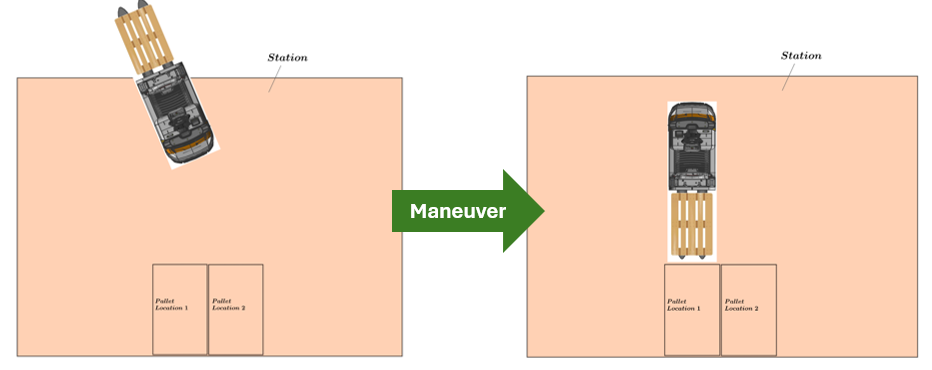
\includegraphics[width=1.0\linewidth]{maneuver.png}
  \caption{Need to maneuver for target docking}
  \label{maneuver}
\end{figure}
%#######################################################################

The proposed methodology consists of several key components that work together to ensure real-time path generation and optimization:
\subsection{Geometric Partitioning}
The warehouse is divided into predefined zones, ensuring the robot can adaptively plan movements between them. Each station is represented as a structured area where path linking would be optimized.
Each station has a shelf to store the handled materials. The station is partitioned, according to its layout,
into two free zones to serve as maneuver zones labeled on figure \ref{geometric_partitioning} as "transition polygons".

%#######################################################################
\begin{figure}[t]
  \centering 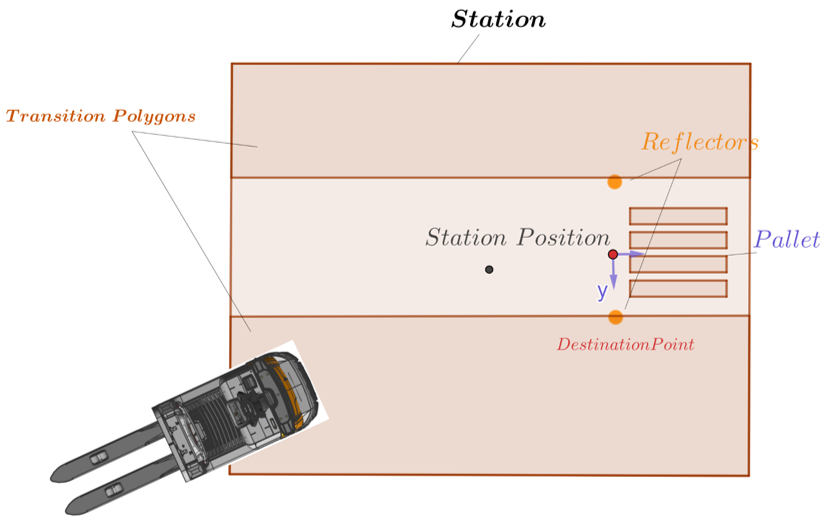
\includegraphics[width=1.0\linewidth]{geometric_partitioning.png}
  \caption{Station Model with shelf, a forklift, and the transition polygons \cite{ref2}}
  \label{geometric_partitioning}
\end{figure}
%#######################################################################

\subsection{Pattern-Based Path Creation}
The transition polygons are then used to maneuver: a transition position is set and through it, the AMR stops briefly to drive in the opposite direction. The pattern path is visible in figure \ref{pattern path}.

\begin{figure}[t]
  \centering 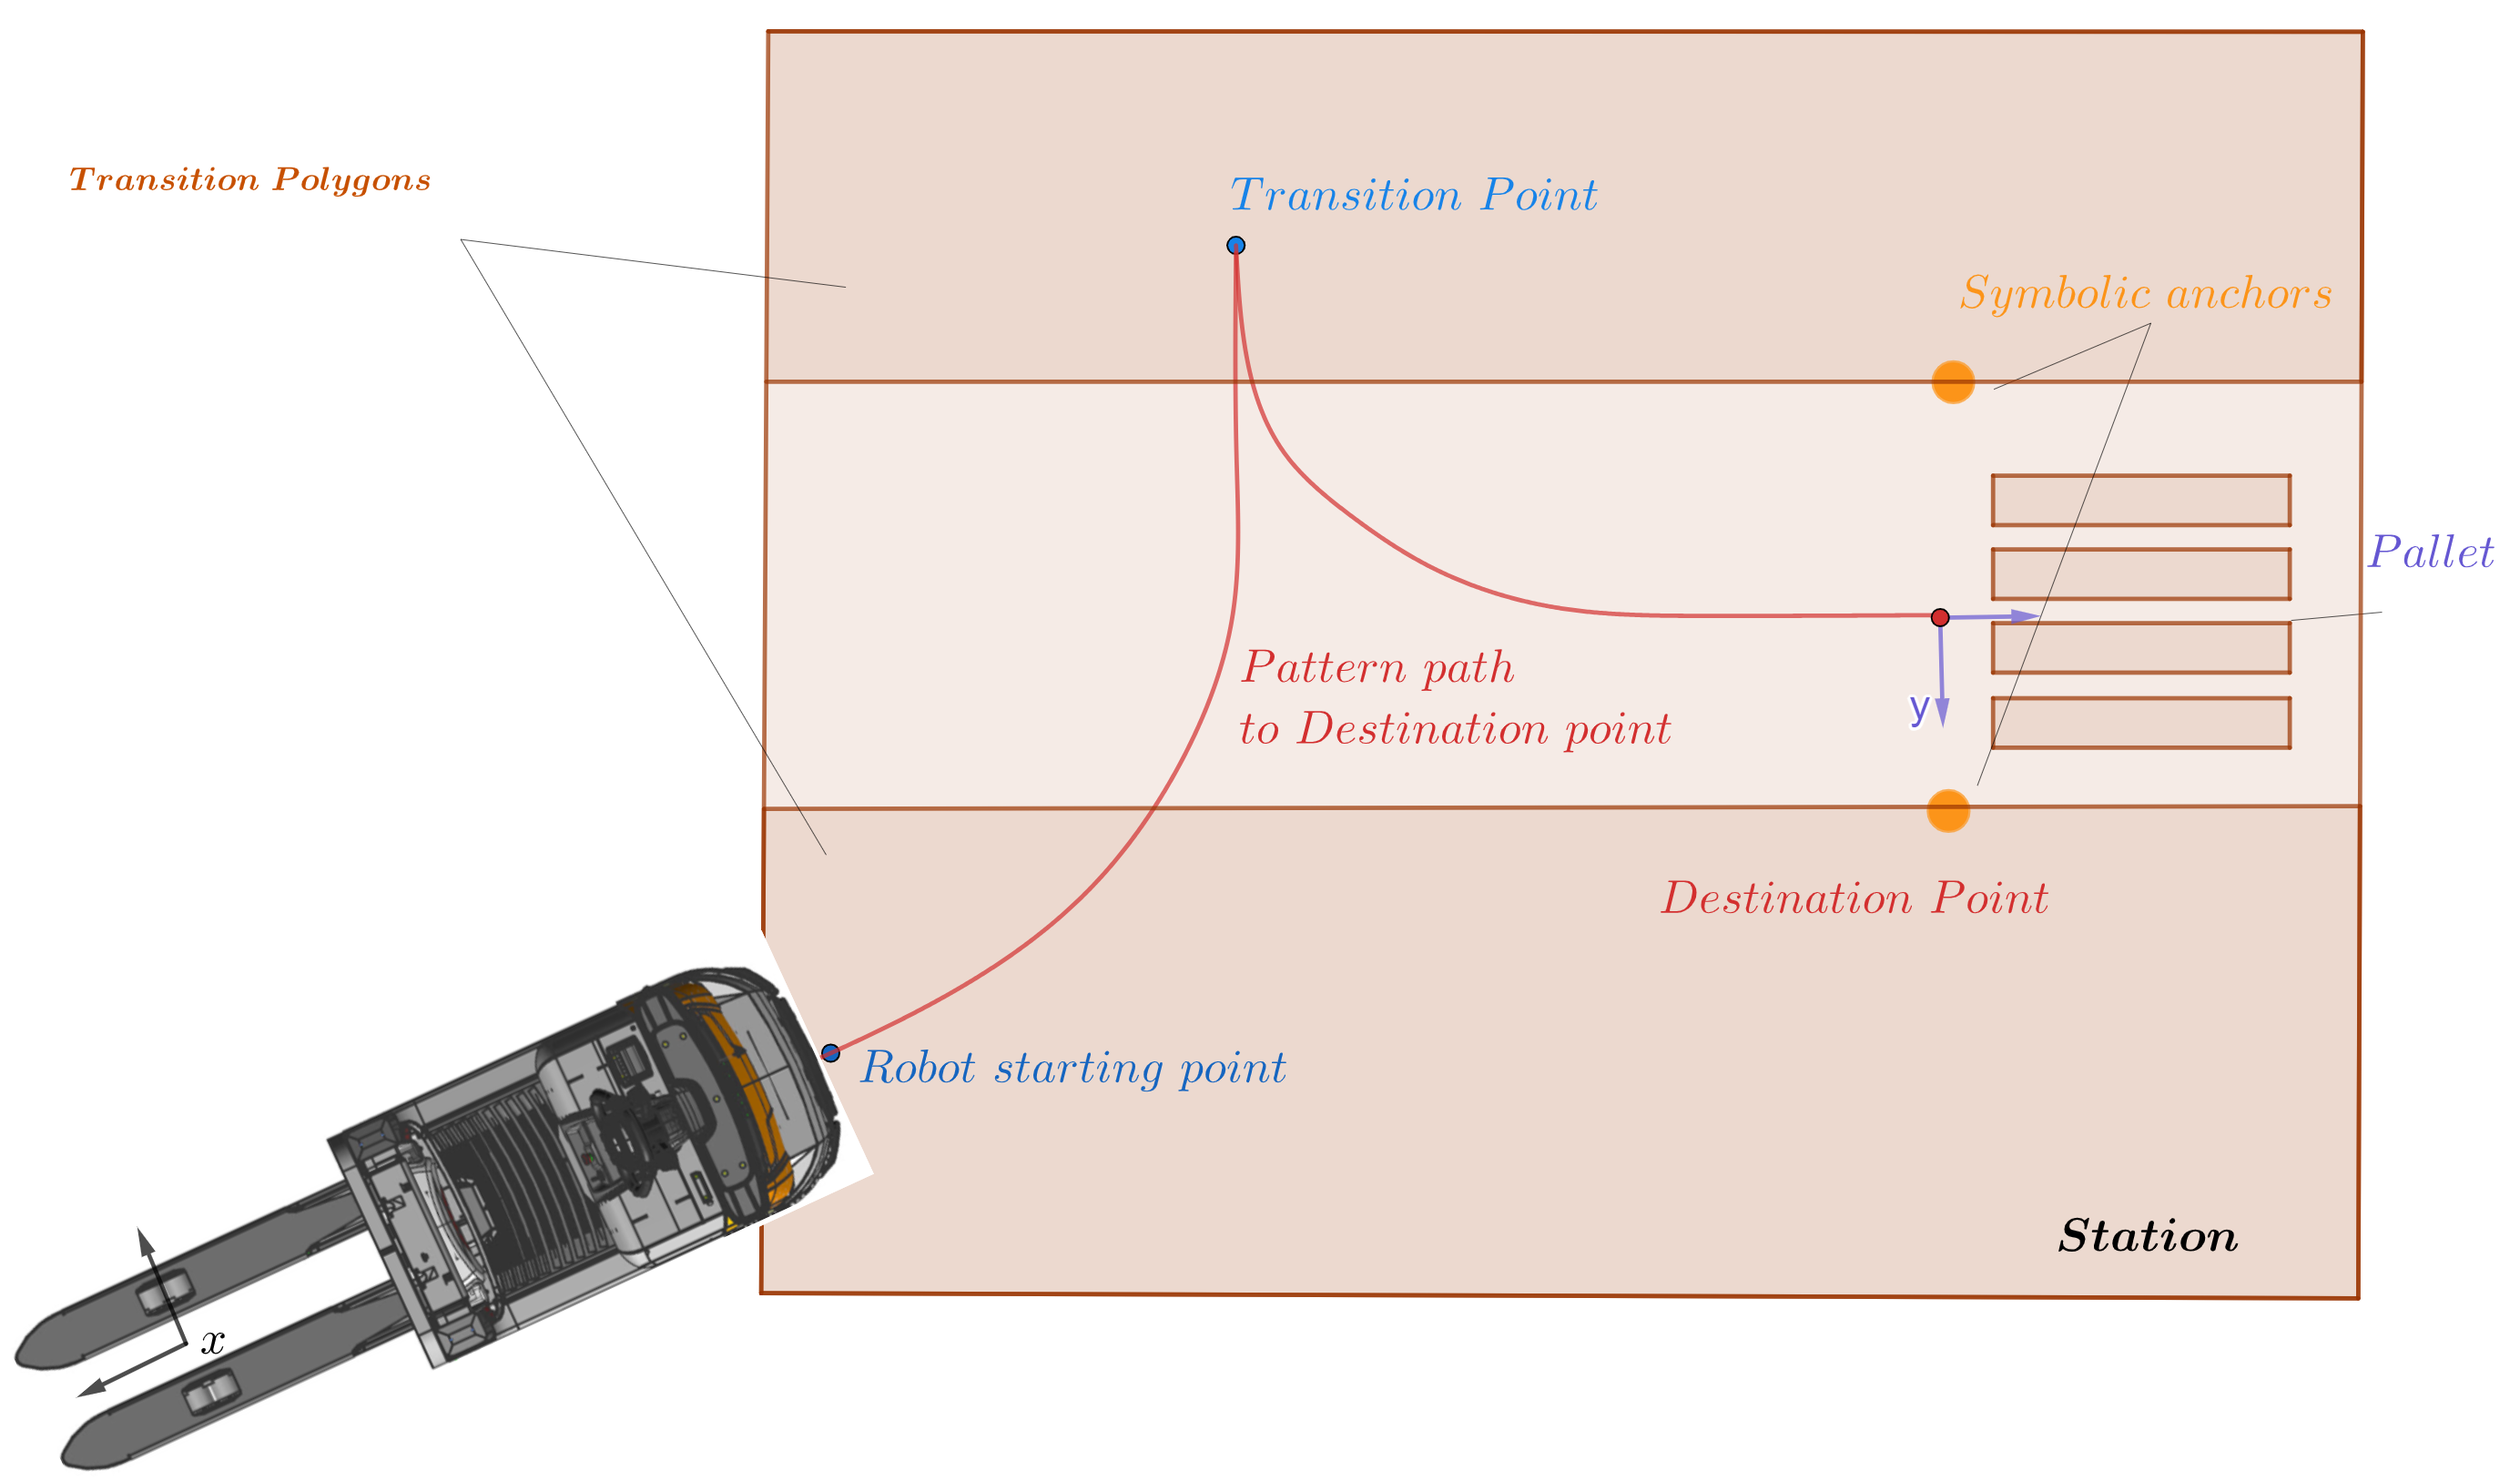
\includegraphics[width=1.0\linewidth]{PatternPathComplFigure.png}
  \caption{Pattern path, linking the start position to the target, passing through a transition position to change directions \cite{ref2}}
  \label{pattern path}
\end{figure}

The approach leverages splines to generate smooth paths between waypoints, ensuring high kinematic feasibility through continuous speed and acceleration.
\subsection{Path Evaluation Metrics}
Several evaluation criteria are implemented to assess path efficiency, including curvature change minimization to prevent abrupt changes in steering and unfeasible curves, travel distance, and obstacle avoidance. First colliding paths are omitted, then the paths are discriminated by their quality. Using the developed cost function, each path's quality is quantified by a value measured using a cost function. The smaller the value, the better the path.

\begin{equation}
    CF= \omega_{C} \cdot \underbrace{\frac{\sum_{i=\text{j min par}}^{\text{j max par}} 
    \frac{\Delta k(i)_j}{\Delta s(i)_j}}{\sum_{i=\text{ref min par}}^{\text{ref max par}} 
    \frac{\Delta k(i)_{\text{ref}}}{\Delta s(i)_{\text{ref}}}}}_{\text{C}} 
    + \omega_{L} \cdot \underbrace{\frac{\sum_{i=\text{min par}}^{\text{max par}} s(i)_j}
    {\sum_{i=\text{min par}}^{\text{max par}} s(i)_{\text{ref}}}}_{\text{D}}
    \label{Norm_function}
\end{equation}

\noindent Where:

\noindent - \(\omega_c\) and \(\omega_L\) are the weights assigned to the curvature change term and the length term, 
    respectively. These weights determine the relative importance of curvature change and path length in the overall evaluation. 
\newline - C is the Curvature Change Term.
\newline - D is the Length Term.

These terms are normalized by division by a reference value of a random path and weighted to control the influence of each term on the outcome, then summed \cite{ref3}.

\subsection{Meta-heuristic Optimization}
Various optimization techniques, such as genetic algorithms (GA), Ant Colony Optimization (ACO), and particle swarm optimization (PSO), are used to refine path selection and dynamically adapt to new environmental constraints. The algorithms were integrated using the PAGMO library and the minimization of the cost function as an objective function.
\subsection{Obstacle Avoidance}
The system uses the B-Splines property of interpolating new waypoints without affecting the general shapes of the curve. In case of obstacles, the algorithms sets waypoints that influence that path to stray away from them. 
\subsection{Implementation in RACK Framework}
The Robotics Application Construction Kit (RACK) is used to validate the approach through simulation then real-world deployment in a warehouse setting.


%############################
\section{Experimental Results and Discussion}
The proposed approach was rigorously tested in simulation and real-world scenarios, validating its efficiency, reliability, and adaptability. The results confirm that the system efficiently generates optimized, explainable, and collision-free paths in minimal time.

\noindent \textbf{Path Creation and Validation:} The pattern-based approach successfully generated smooth, kinematically feasible paths that adhered to warehouse constraints and linked the AMR in start position to the specified target. Tests in both simulation and real-world environments confirmed the effectiveness of transition points in reducing curvature and improving maneuverability. An overview of a situation with an obstacle in the environment is visible in figure \ref{obstacle}. 

%#######################################################################
\begin{figure}[t]
  \centering 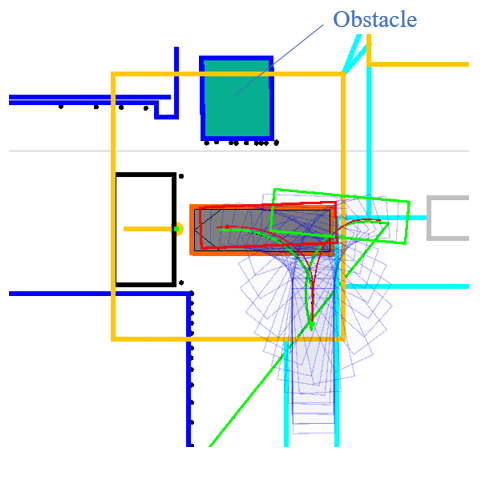
\includegraphics[width=3in]{obstacle_complicated.png}
  \caption{Simulation environment of a complex situation overview inside a station (yellow frame) with initial position (green frame), target position (red frame), generated path (green), and obstacle (green square) }
  \label{obstacle}
\end{figure}
%#######################################################################

\noindent \textbf{Path Evaluation and Optimization:} 
Tests in simple and complex environment settings were executed using the 
RACK Simulation Environment to compare the performance of the Meta-heuristic algorithms: Genetic Algorithms (GA), Differential Evolution (DE), Particle Swarm Optimization (PSO), Ant Colony Optimization (ACO), and Simulated Annealing (SA). After each processing of the situation and test environment the best feasible path among all the generated ones is saved as the champion path. 
A comparative analysis of the algorithms based on fitness values of the champion paths and planning time demonstrated that PSO provided the most balanced performance in terms of planning time and path quality. The selected evaluation method effectively discriminated between high- and low-quality paths, ensuring optimal trajectory selection.  

\noindent \textbf{Performance Metrics:} The solution demonstrated significant improvements in computational efficiency, achieving path planning times as low as 59ms in simple environments and 67ms in complex scenarios. Real-world execution times remained within acceptable limits, validating the approach’s practicality.

These results highlight the robustness of the proposed solution in optimizing AMR path planning while maintaining high levels of explainability and adaptability.

\section{Conclusion and Future Work}
This research presents an optimized path-planning approach for Autonomous Mobile Robots (AMRs), focusing on repeatable, station-specific paths that ensure precise docking. The method integrates metaheuristic optimization to minimize path length and curvature while adhering to kinematic constraints. Unlike traditional approaches, which suffer from high computational costs and long planning times (13–31 s), this solution achieves significantly faster results: 40–50 ms in simulation and a maximum of 400 ms in real-world tests.

The approach enhances explainability and predictability by generating human-interpretable paths, with well-defined optimization parameters. It also improves adaptability, allowing seamless deployment in varying station layouts. Field tests confirm the method’s robustness, demonstrating its practical applicability in real-world AMR operations. Looking ahead, this research can be refined by integrating more transition zones to improve the exploration of the entire free space within the station and optimizing the use of transition polygons based on the AMR’s position to reduce the risk of low-quality reference points and generated paths. Additionally, further work can focus on documenting the findings in a scientific article to contribute to the field and enhance knowledge dissemination. These refinements will improve the approach’s efficiency, adaptability, and practical implementation in industrial robotics applications.

%\section{References}
\begin{thebibliography}{9}
\bibitem{ref1} S. Alaliyat, R. Oucheikh and I. Hameed, "Path Planning in Dynamic Environment Using Particle Swarm Optimization Algorithm," 2019 8th International Conference on Modeling Simulation and Applied Optimization (ICMSAO), Manama, Bahrain, 2019.
\bibitem{ref2} Kr\"uger-Basjmeleh, T. (2024). Bef\"ahigung autonomer, mobiler roboter zum one-shot-imitationslernen f\"ur 
Den vollst\"andigen transport von paletten in lager- und produktionsbereichen Tino Kr\"uger-Basjmeleh. Verlag Dr. Hut.
\bibitem{ref3} A. Elshamli, H. A. Abdullah and S. Areibi, "Genetic algorithm for dynamic path planning," Canadian Conference on Electrical and Computer Engineering 2004 (IEEE Cat. No.04CH37513), 
Niagara Falls, ON, Canada, 2004.
\end{thebibliography}

\end{document}
